\chapter{实验结果分析}
\section{算法总体性能测试}

本次测试所用的矩阵主要来自于\cite{park2014sparsifying}和\cite{liuSyncFree2016}这两篇文章中所用到的矩阵,这些矩阵都可以从MatrixMarket和弗罗里达大学稀疏矩阵集合中下载。本次测试所使用的矩阵如表\ref{MatrixSuite}所示。表中最后一列并行性的定义为并行性=矩阵的行数$ \div $最大level数,可以理解为平均每个level有多少的任务即可,其中并行性最好的是矩阵是nlpkkt160,只有两个level,理论并行性最差的是af\_shell10和chipcool0。

\begin{table}[htbp]
    \scriptsize
    \caption{性能测试所用矩阵}
    \label{MatrixSuite}
    \resizebox{\textwidth}{!}{%
    \begin{tabular}{|l|r|r|r|r|}
    \hline
    矩阵名称 & 行或列数量 & 非零元个数 & 最大level数 & 并行性 \\ \hline
    nlpkkt160     & 8,345,600     & 229,518,112   & 2   & 4,172,800   \\
    road\_usa     & 23,947,347    & 57,708,624    & 77  & 311,004     \\
    road\_central & 14,081,816    & 33,866,826    & 59  & 238,674     \\
    wiki-Talk     & 2,394,385     & 5,021,410     & 522 & 4,586       \\
    webbase-1M    & 1,000,005     & 3,105,536     & 514 & 1,945       \\
    apache2       & 715,176       & 4,817,870     & 664 & 1,077       \\
    thermal2      & 1,228,045     & 8,580,313    & 1,239& 991        \\
    G3\_circuit   & 1,585,478     & 7,660,826    & 2,594& 611         \\
    StocF-1465    & 1,465,137     & 21,005,389   & 3,004& 487         \\
    af\_shell10   & 1,508,065     & 52,259,885   & 8,360& 180         \\
    chipcool0     & 20,082        & 2,81,150     & 534  & 37          \\ \hline
    \end{tabular}%
    }
\end{table}

实验所用的硬件平台为华为鲲鹏920处理器,4个NUMA结点,每个结点有32个核心以及130GB的内存,结点间带宽为480Gbps。软件平台:操作系统CentOS7.6.1810。编译器gcc9.0。openmp4.5。

首先,图\ref{在多个稀疏矩阵上的测试数据}展示了在11个稀疏矩阵下的性能测试数据,绝大多数的矩阵都能够获得2倍以上的加速比(黄色那条线)。折线图的横坐标为矩阵的名称,按照表\ref{MatrixSuite}中,矩阵的并行性从高到低排序。可以看出,矩阵并行性越高,加速比越高。

\begin{figure}[htbp]
    \centering
    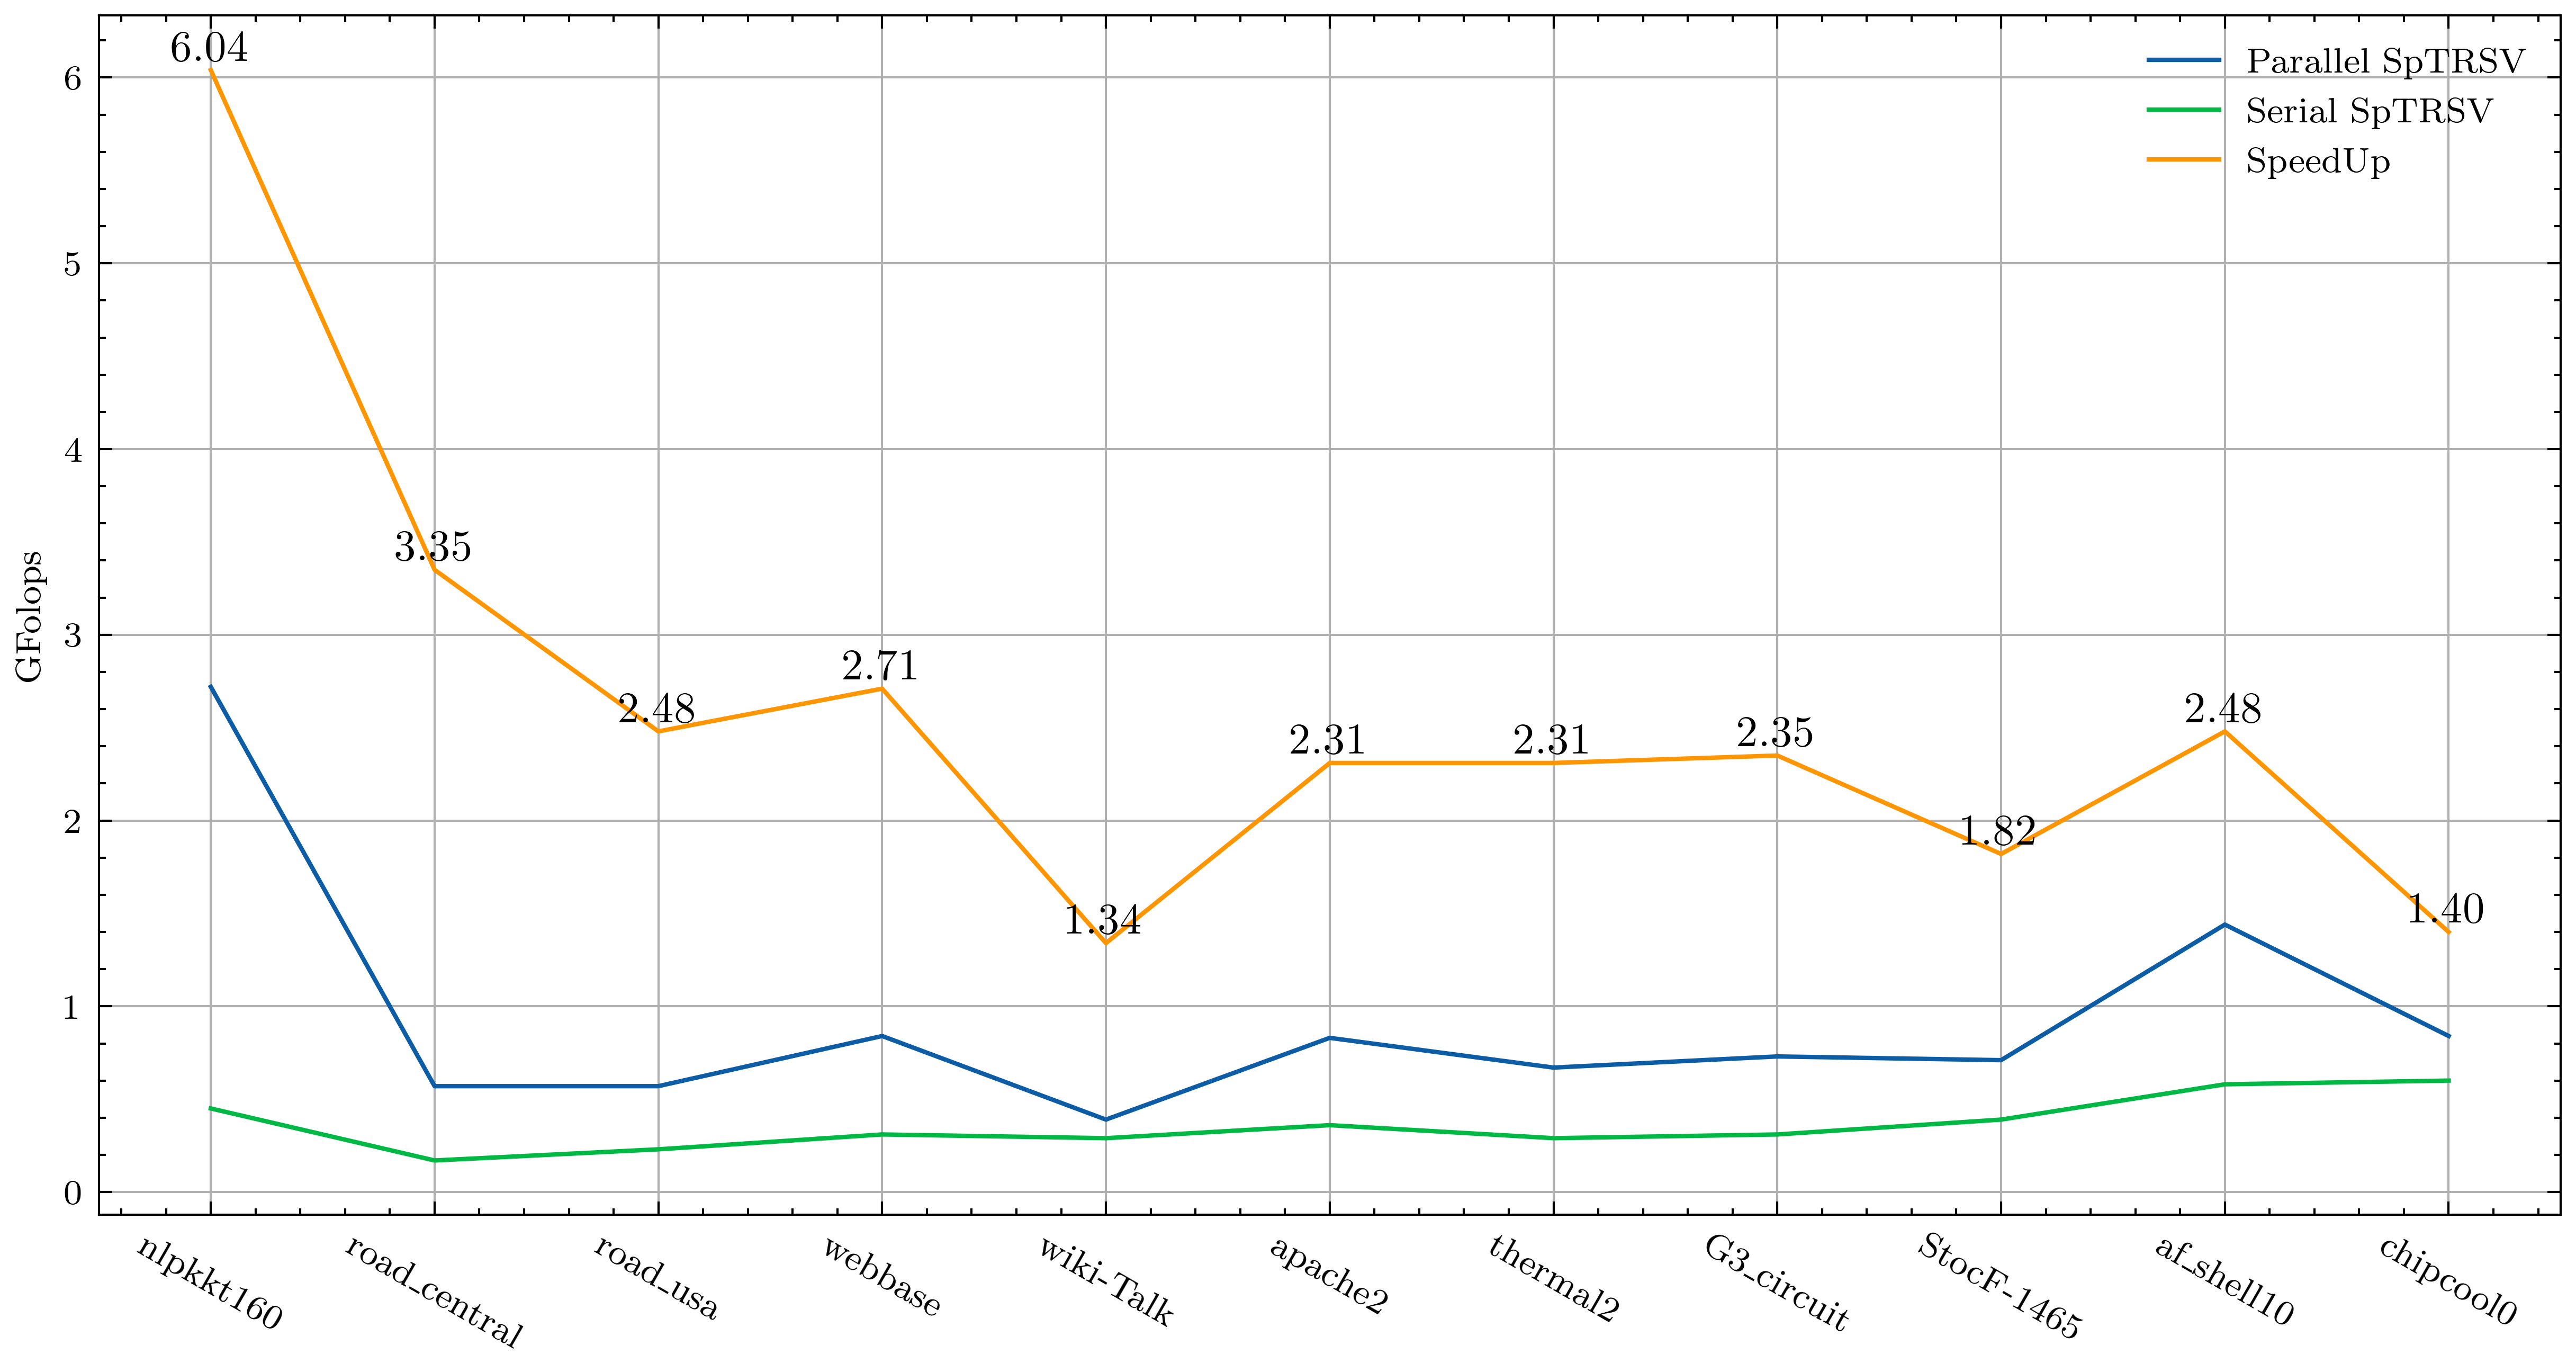
\includegraphics[width=0.9\textwidth]{moreData.png}
    \caption{在多个稀疏矩阵上的测试数据}
    \label{在多个稀疏矩阵上的测试数据}
\end{figure}

~\\

% 然后,将本文提出的SpTRSV算法与intel MKL数学库中的SpTRSV算法进行了性能对比,结果如图\ref{SpTRSVMulti-paltform}所示,intel平台采用CPU双路志强E5-2695v3 14x2个核心,130GB内存,MKL版本为11.3。柱状图从左到右依次为:MKL数学库中串行算法的性能、并行算法的性能;在鲲鹏920处理器上,使用本文提出的串行算法的性能、并行算法的性能;纵轴以Gflops为单位来衡量算法的性能。Gflops计算方法为$(2 \times NNZL)  \div totoal\_time$。$totoal\_time = preprocess\_time + calculate\_time$。NNZL表示下三角矩阵非零元的个数,采用双精度浮点类型,所以前面乘2。6张图分别对应6个稀疏矩阵。

% 可以看出,对于并行性较好的矩阵,如nlpkkt160和road\_central,并行算法取得了相比于串性算法3倍以上的加速比。而对于那些并行性较差的矩阵如wiki-Talk以及chipcool0,由于level数量较多,能够获得有限的加速比。

% \begin{figure}[htbp]
%     \centering
%     \subfigure{
%     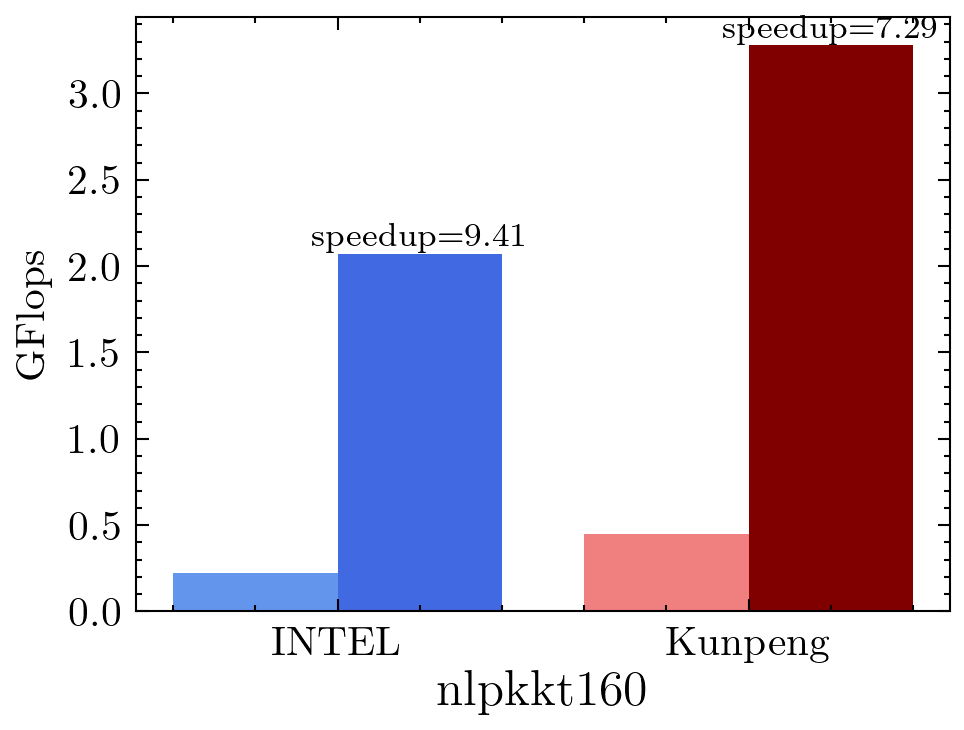
\includegraphics[width=6.5cm]{result0.png}
%     }
%     \quad
%     \subfigure{
%     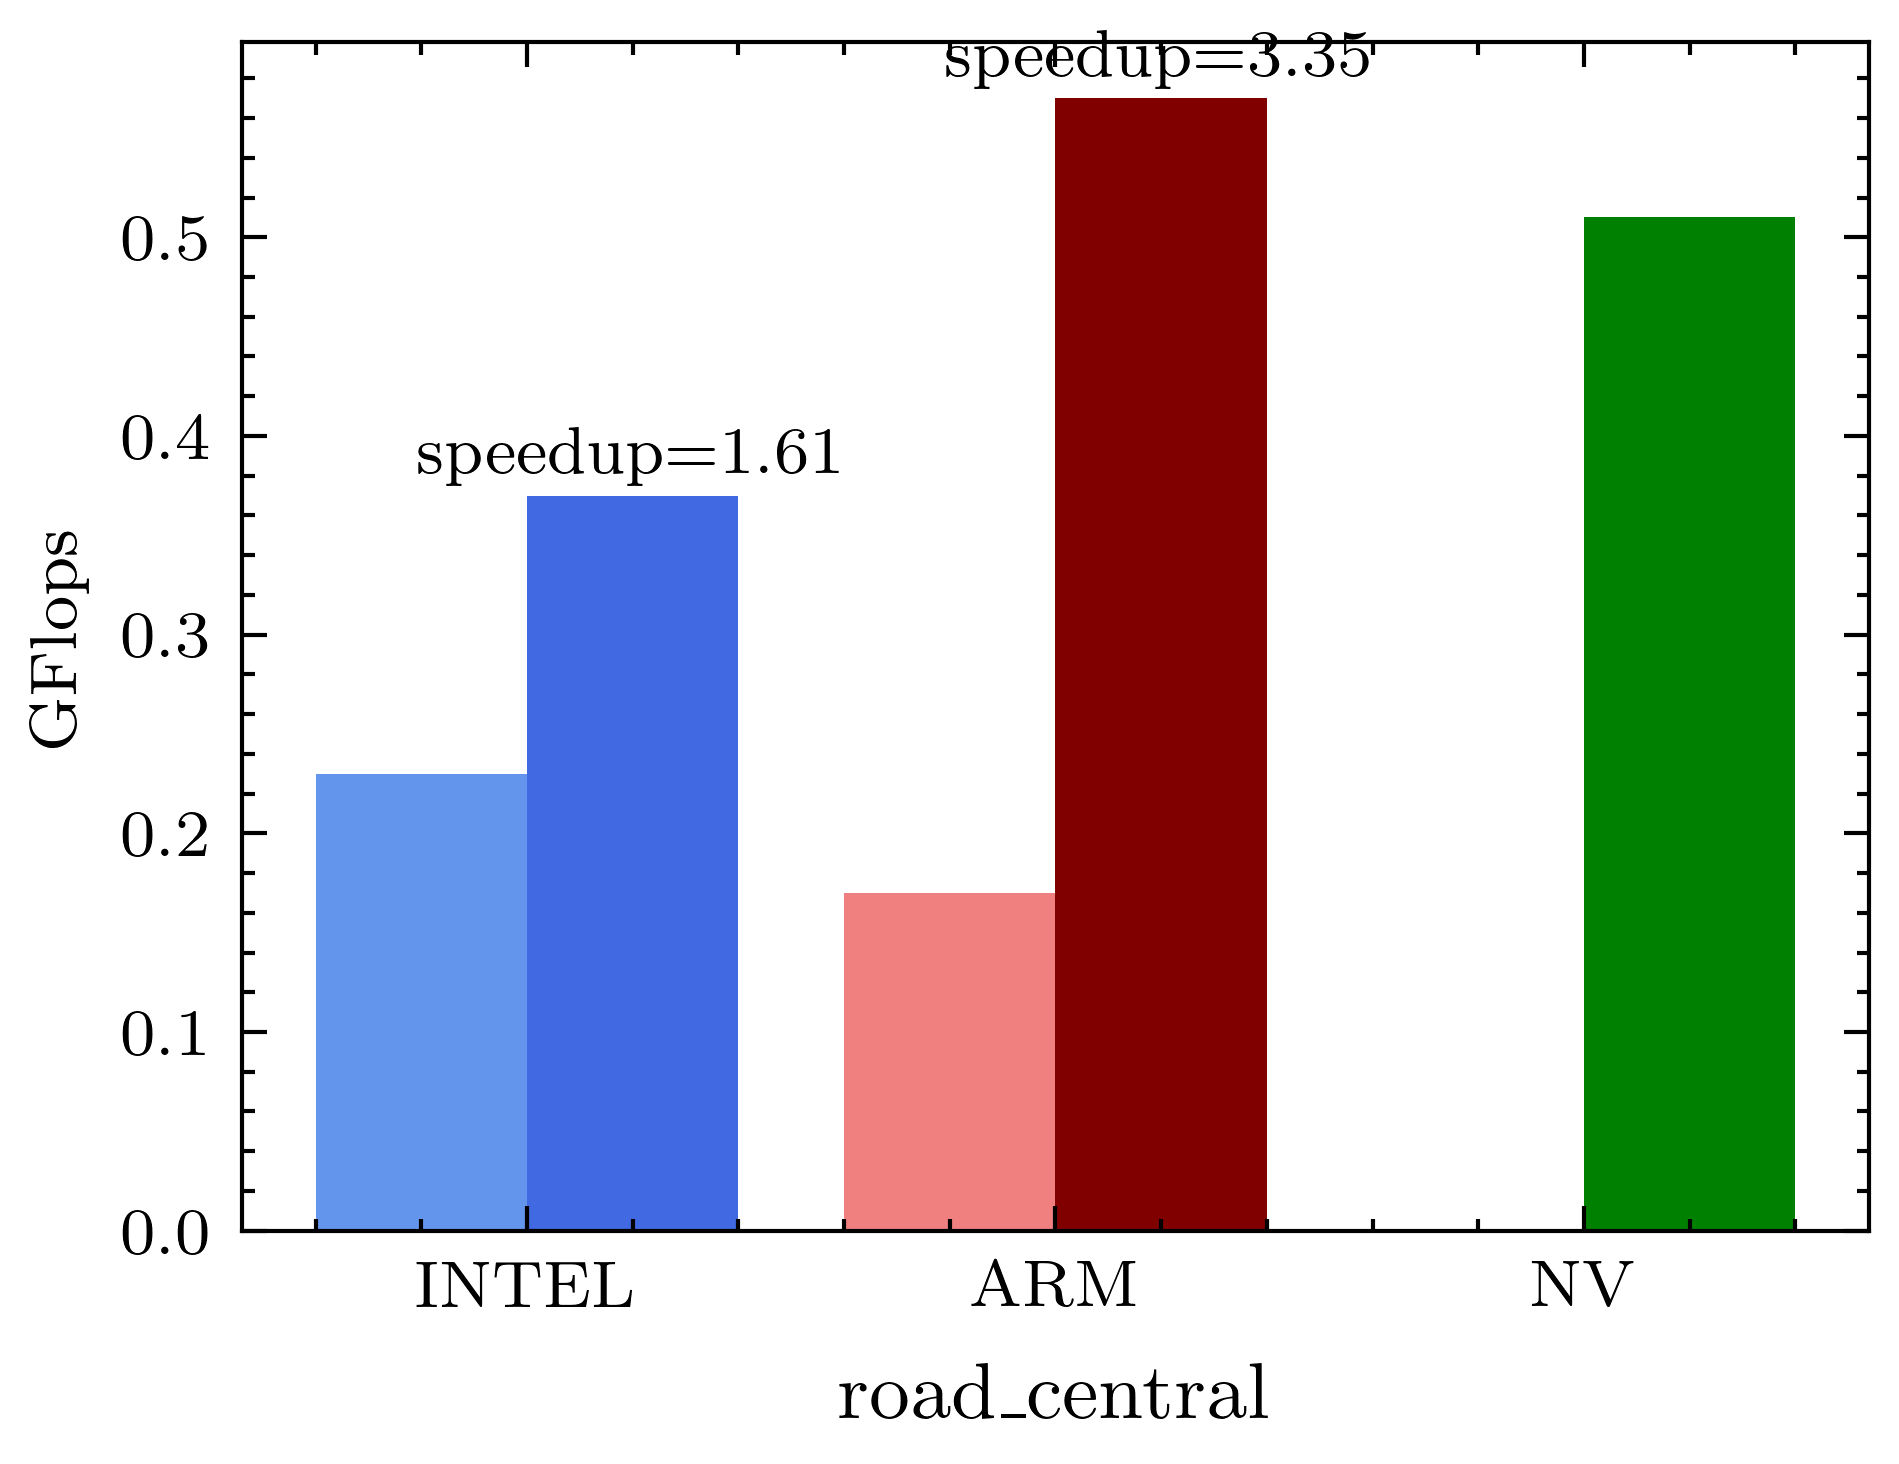
\includegraphics[width=6.5cm]{result1.png}
%     }
%     \quad
%     \subfigure{
%     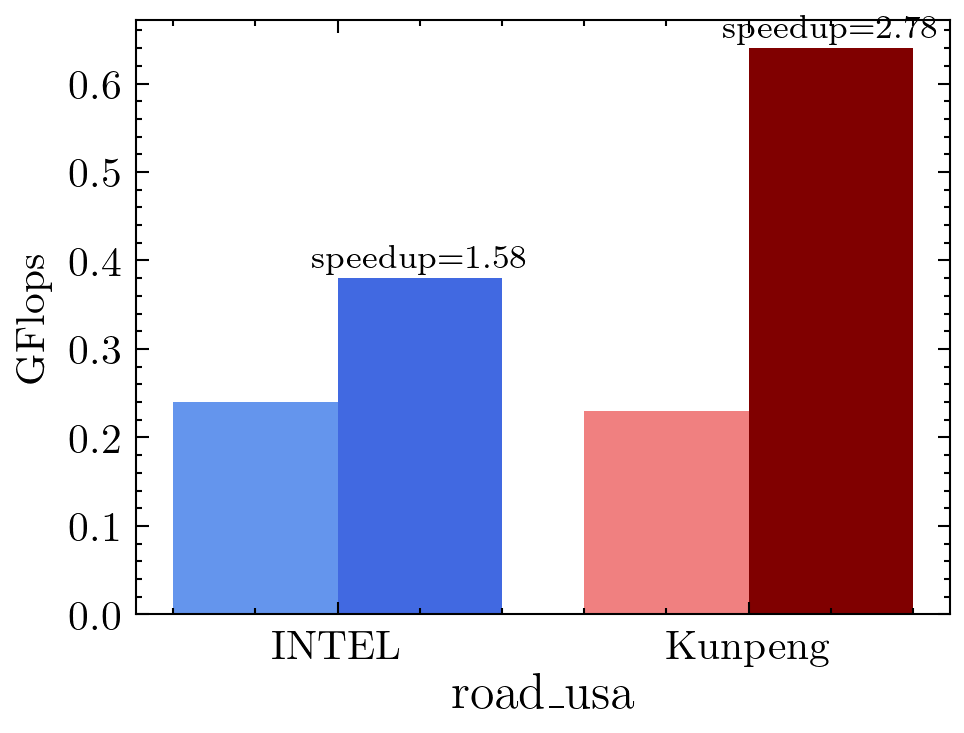
\includegraphics[width=6.5cm]{result2.png}
%     }
%     \quad
%     \subfigure{
%     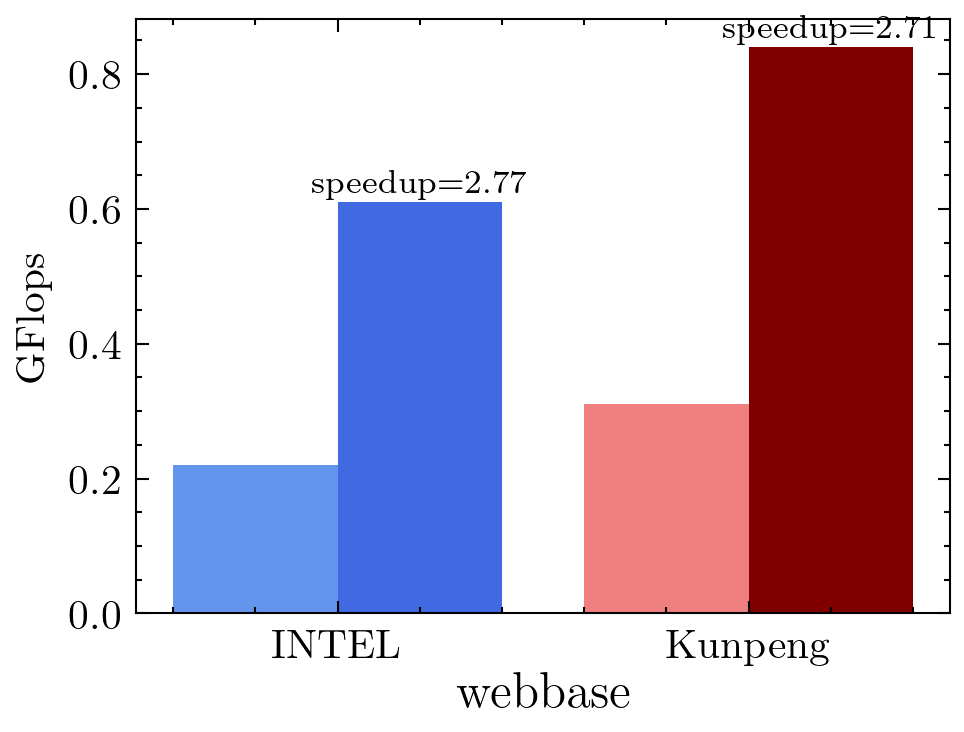
\includegraphics[width=6.5cm]{result3.png}
%     }
%     \quad
%     \subfigure{
%     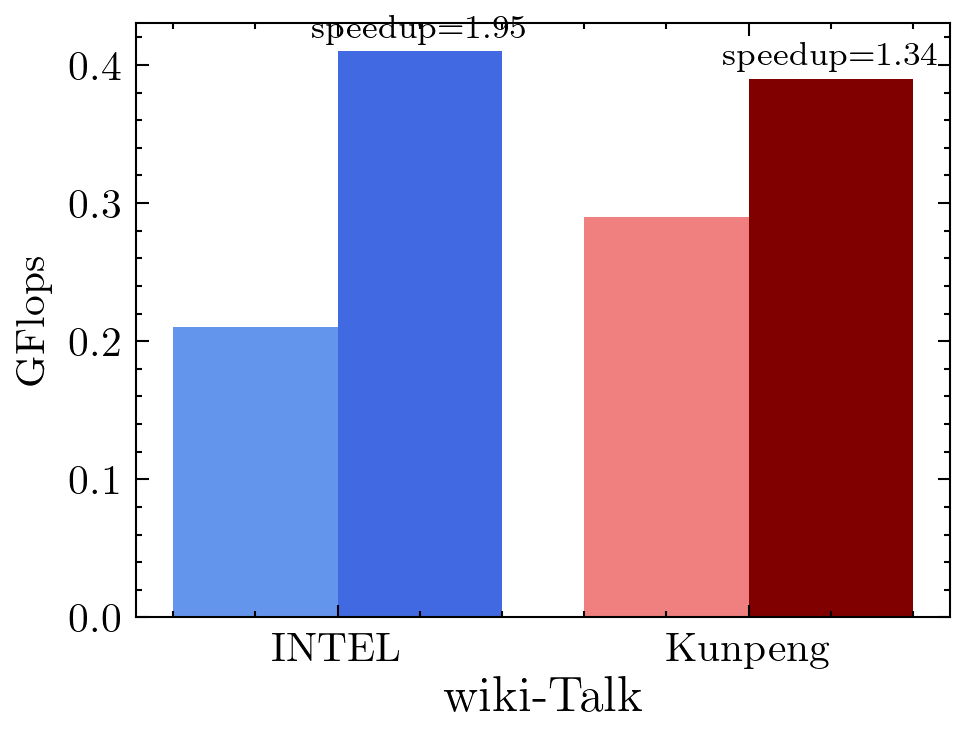
\includegraphics[width=6.5cm]{result4.png}
%     }
%     \quad
%     \subfigure{
%     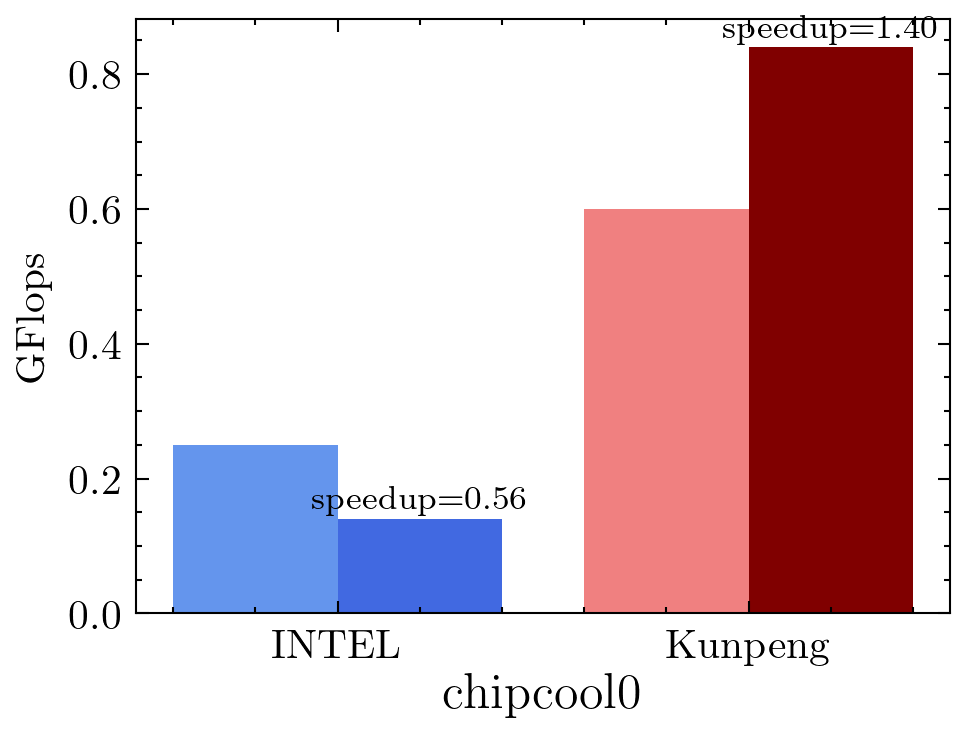
\includegraphics[width=6.5cm]{result5.png}
%     }
%     \caption{本文算法与intel MKL中算法的性能对比}
%     \label{SpTRSVMulti-paltform}
% \end{figure}

\begin{table}[htbp]
    \scriptsize
    \caption{算法耗时分解表}
    \label{算法耗时分解表}
    \resizebox{\textwidth}{!}{%
    \begin{tabular}{|l|r|r|r|r|}
    \hline
    矩阵名称         & 预处理时间(ms) & 计算消耗时间(ms) & 总时间(ms) & 预处理时间占总时间的比例 \\ \hline
    nlpkkt160    & 18.70 & 68.68  & 87.38   & 21.4\%       \\
    road\_central & 20.85 & 87.76  & 108.61  & 19.1\%       \\
    road\_usa     & 42.08 & 141.9  & 77      & 22.8\%       \\
    webbase-1M   & 1.30  & 4.29   & 514     & 23.2\%       \\
    wiki-Talk    & 3.82  & 13.91  & 522     & 21.5\%       \\
    chipcool0    & 0.12  & 0.24   & 534     & 33.3\%       \\ \hline
    \end{tabular}%
    }
\end{table}

如表\ref{算法耗时分解表}所示,算法在预处理阶段主要进行in\_degree的计算,以及通过任务划分的方式进行负载均衡的处理。预处理时间占总时间的20\%左右,且相对稳定。而且,相比于J.Park\cite{park2014sparsifying}基于level-sets的算法(表\ref{任务耗时分解图}),本文的算法在预处理阶的时间消耗很少,例如对于矩阵nlpkkt,基于level-sets的算法需要484.07ms的时间,而本文的算法只需要18.70ms的预处理时间,以及68.68ms的计算时间。


\section{使用负载均衡对性能的提升}

图\ref{测试负载均衡对SpTRSV算法性能的影响}展示了负载均衡操作对算法性能的影响。对于一些任务之间负载相对均衡的矩阵如nlpkkt160,road\_central和road\_usa,负载均衡优化的开启和关闭,并没有很大的影响,相反对于webbase和chipcool,这两个矩阵之间存在着负载不均衡的现象,所以启用负载均衡起到了优化的作用。

\begin{figure}[htbp]
    \centering
    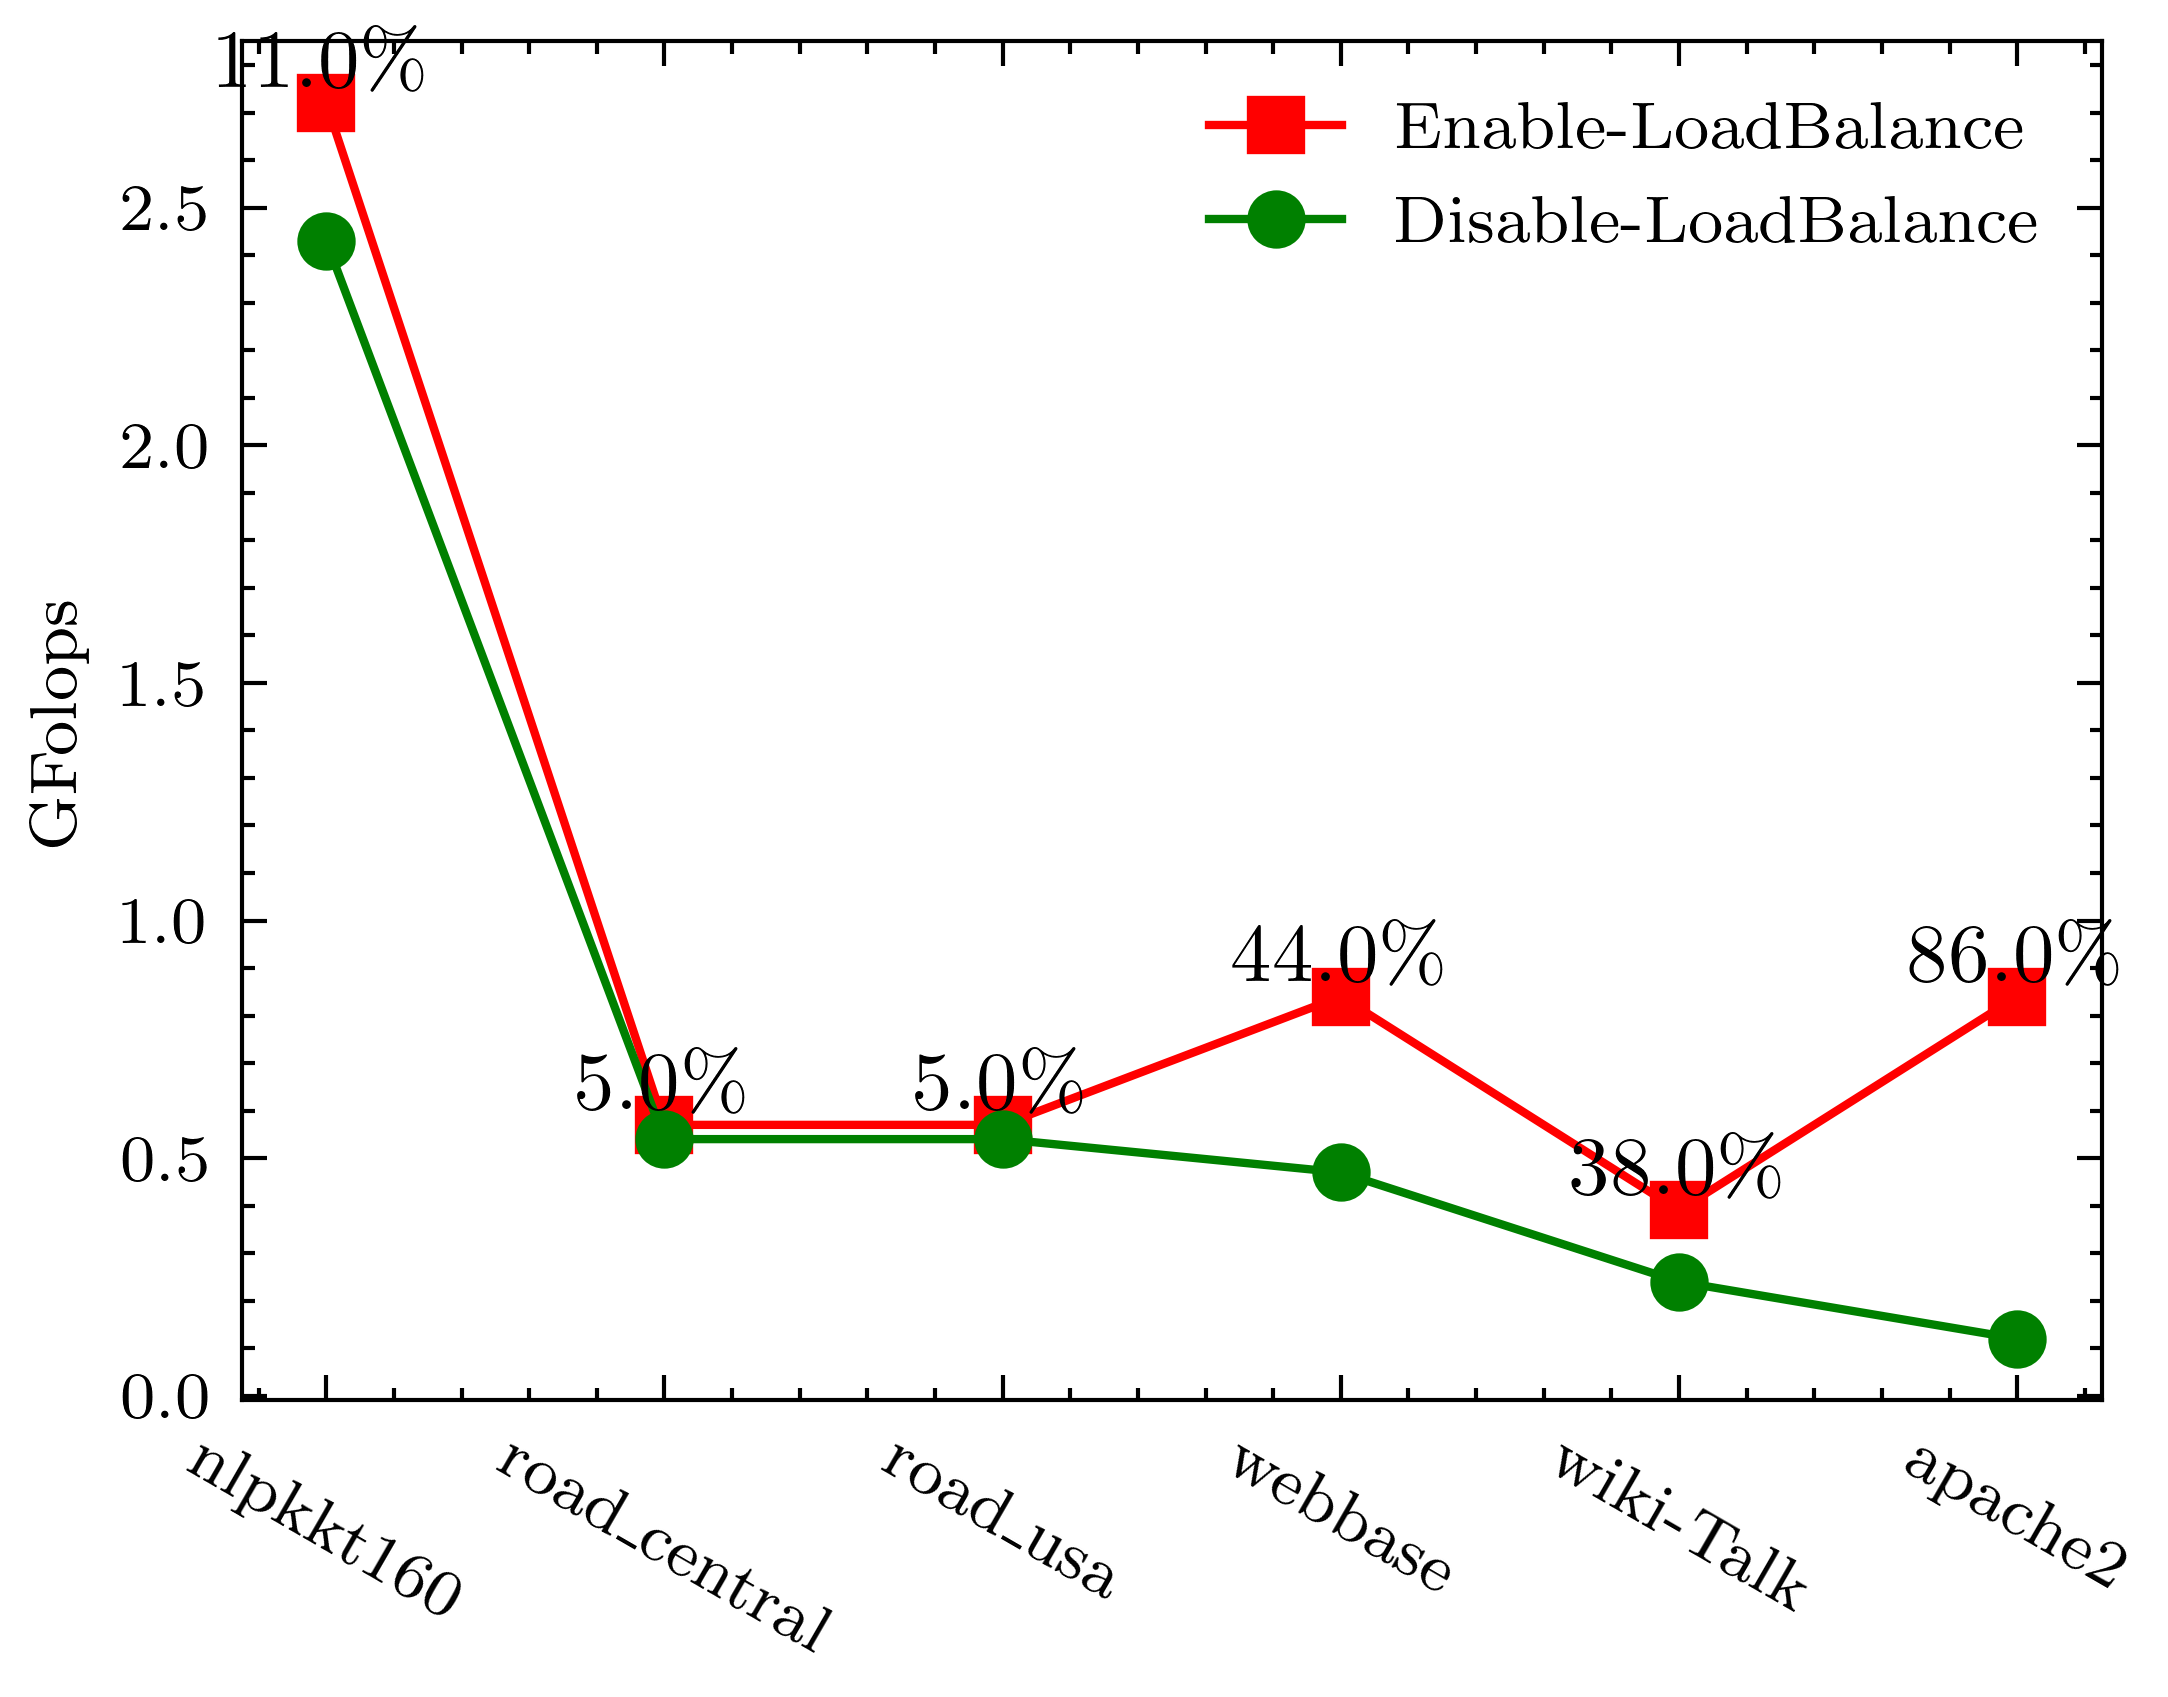
\includegraphics[width=0.7\textwidth]{lbtest.png}
    \caption{测试负载均衡对SpTRSV算法性能的影响}
    \label{测试负载均衡对SpTRSV算法性能的影响}
\end{figure}

\section{使用CPU松弛技术对性能的提升}

\begin{figure}[htbp]
    \centering
    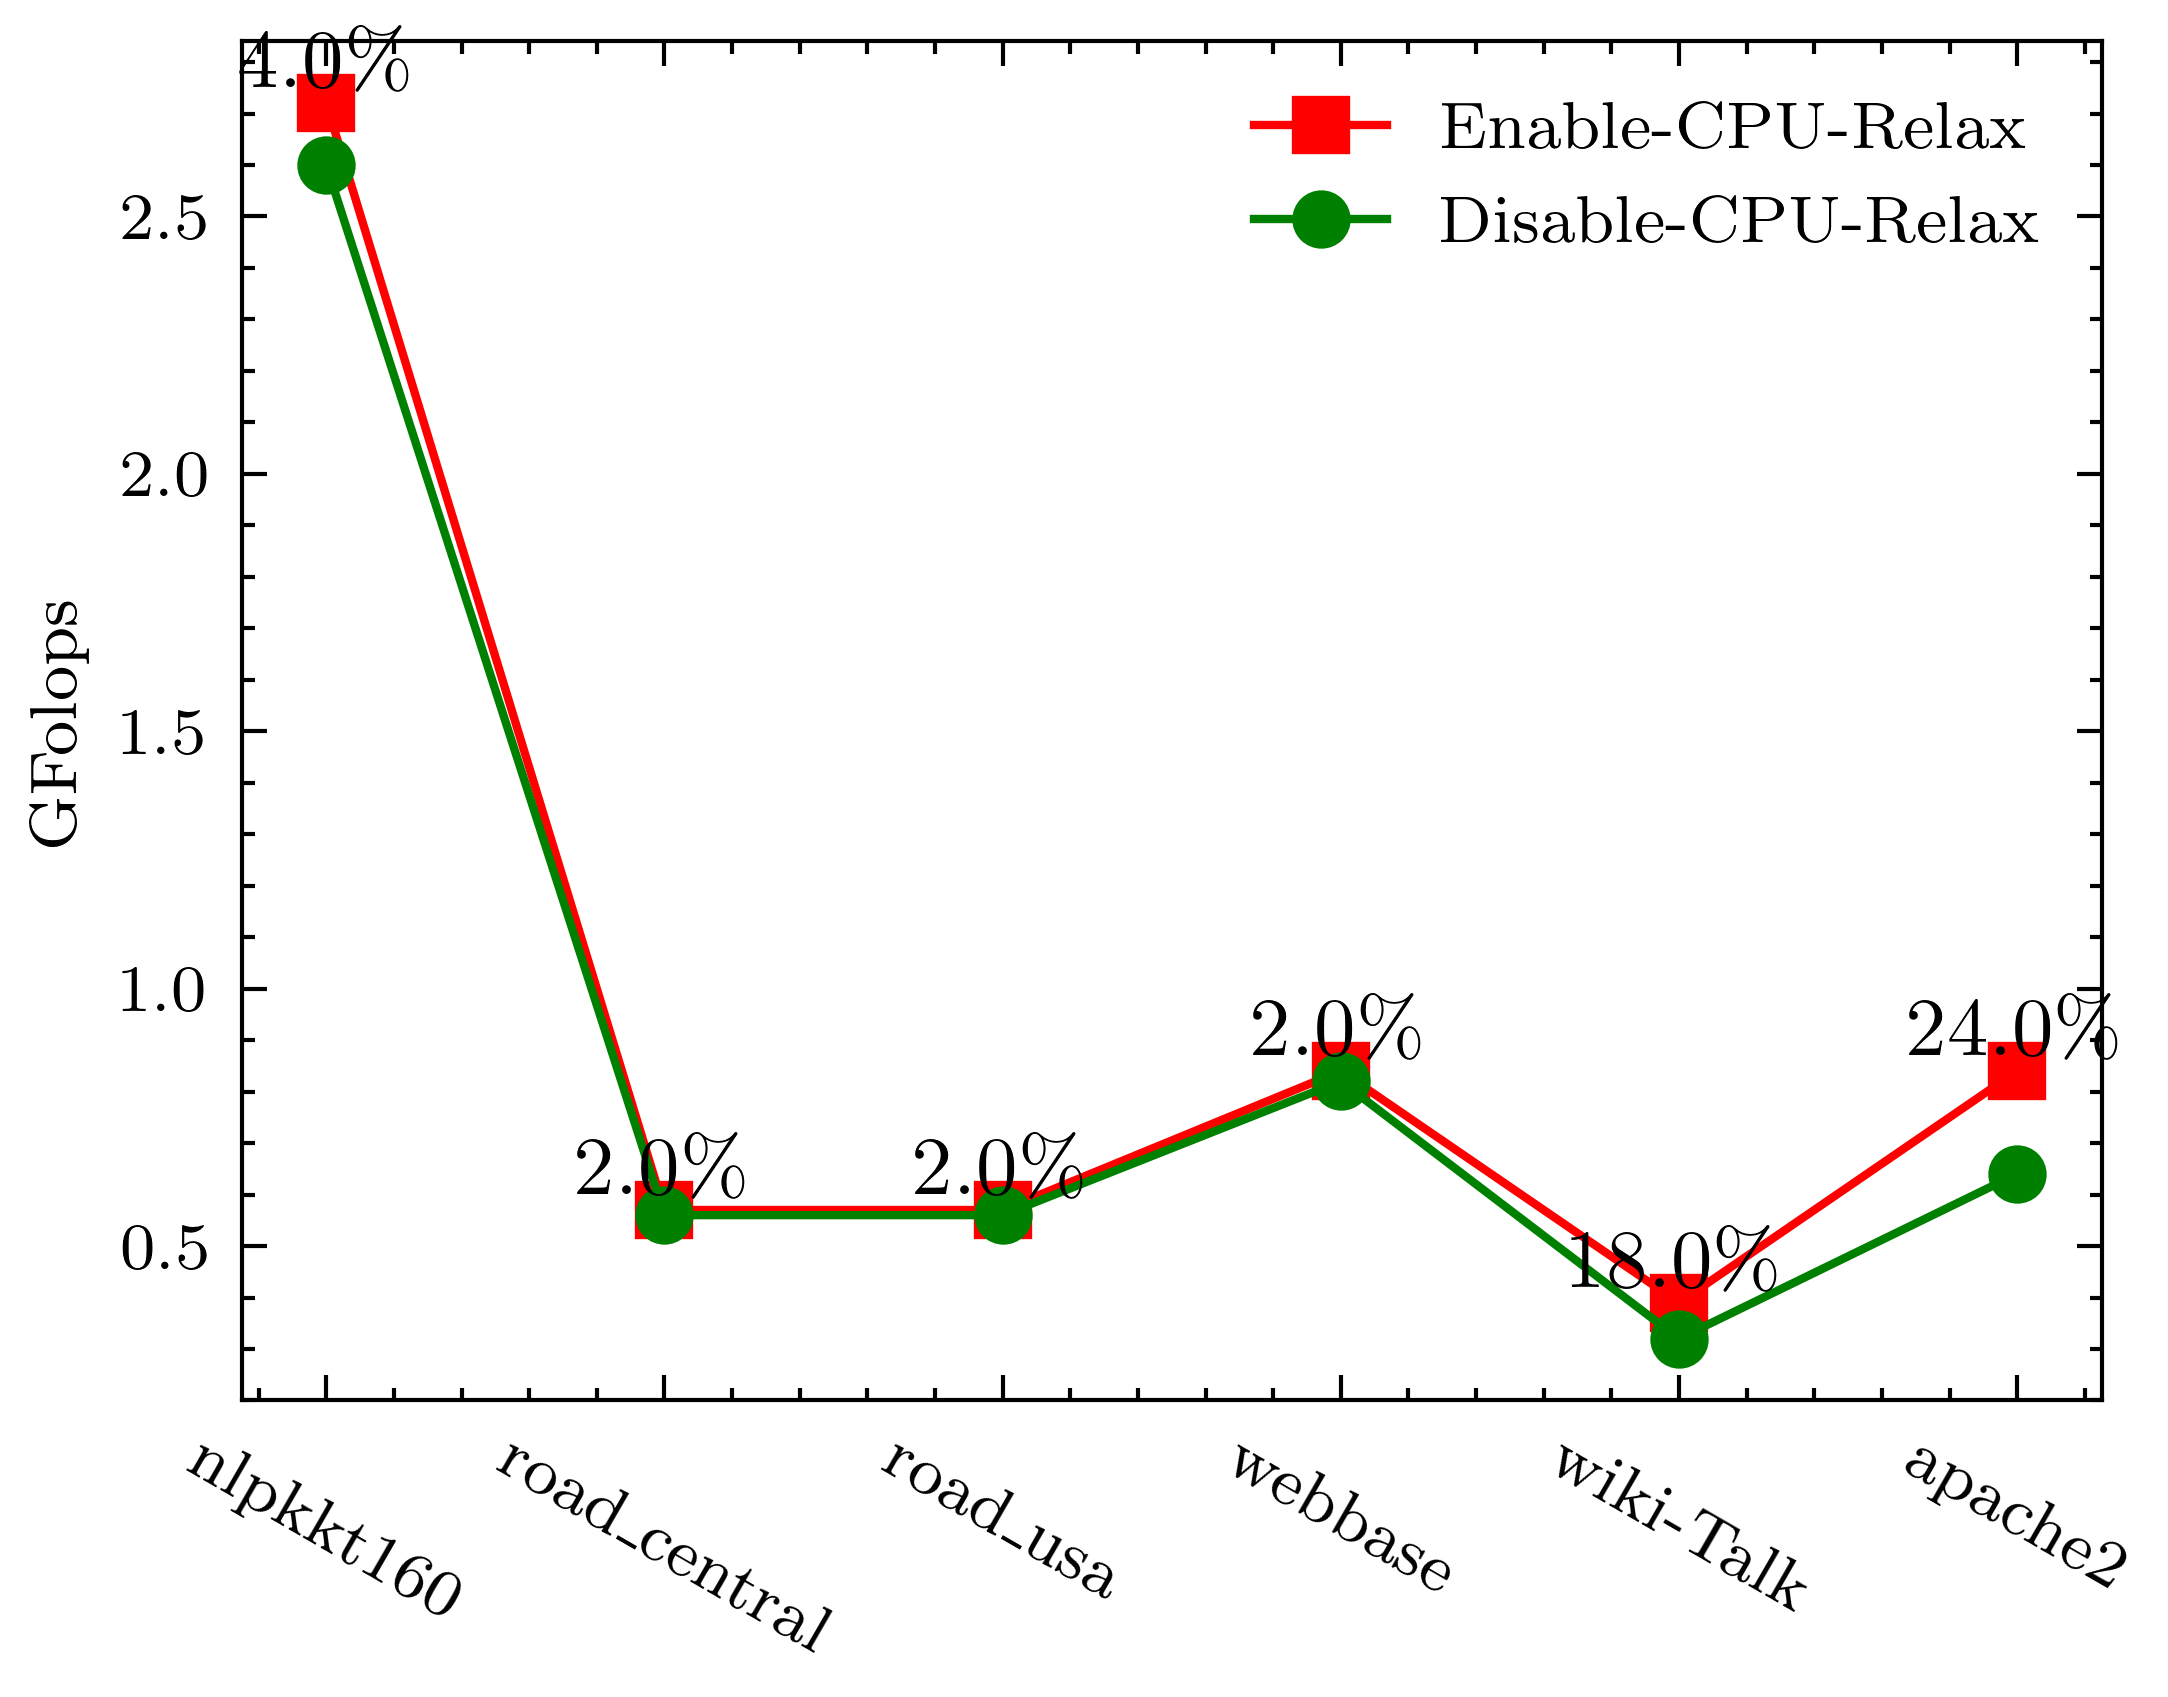
\includegraphics[width=0.7\textwidth]{cpuRelaxTest.png}
    \caption{测试CPU松弛技术对性能的影响}
    \label{测试CPU松弛技术对性能的影响}
\end{figure}

图\ref{测试CPU松弛技术对性能的影响}展示了CPU松弛技术对性能的影响。CPU松弛技术对于一些并行度相对较低的稀疏矩阵有一定的性能提升,总体来说对性能地提升相对较低。

\section{使用ARMv8原子指令对性能的提升}

\begin{figure}[htbp]
    \centering
    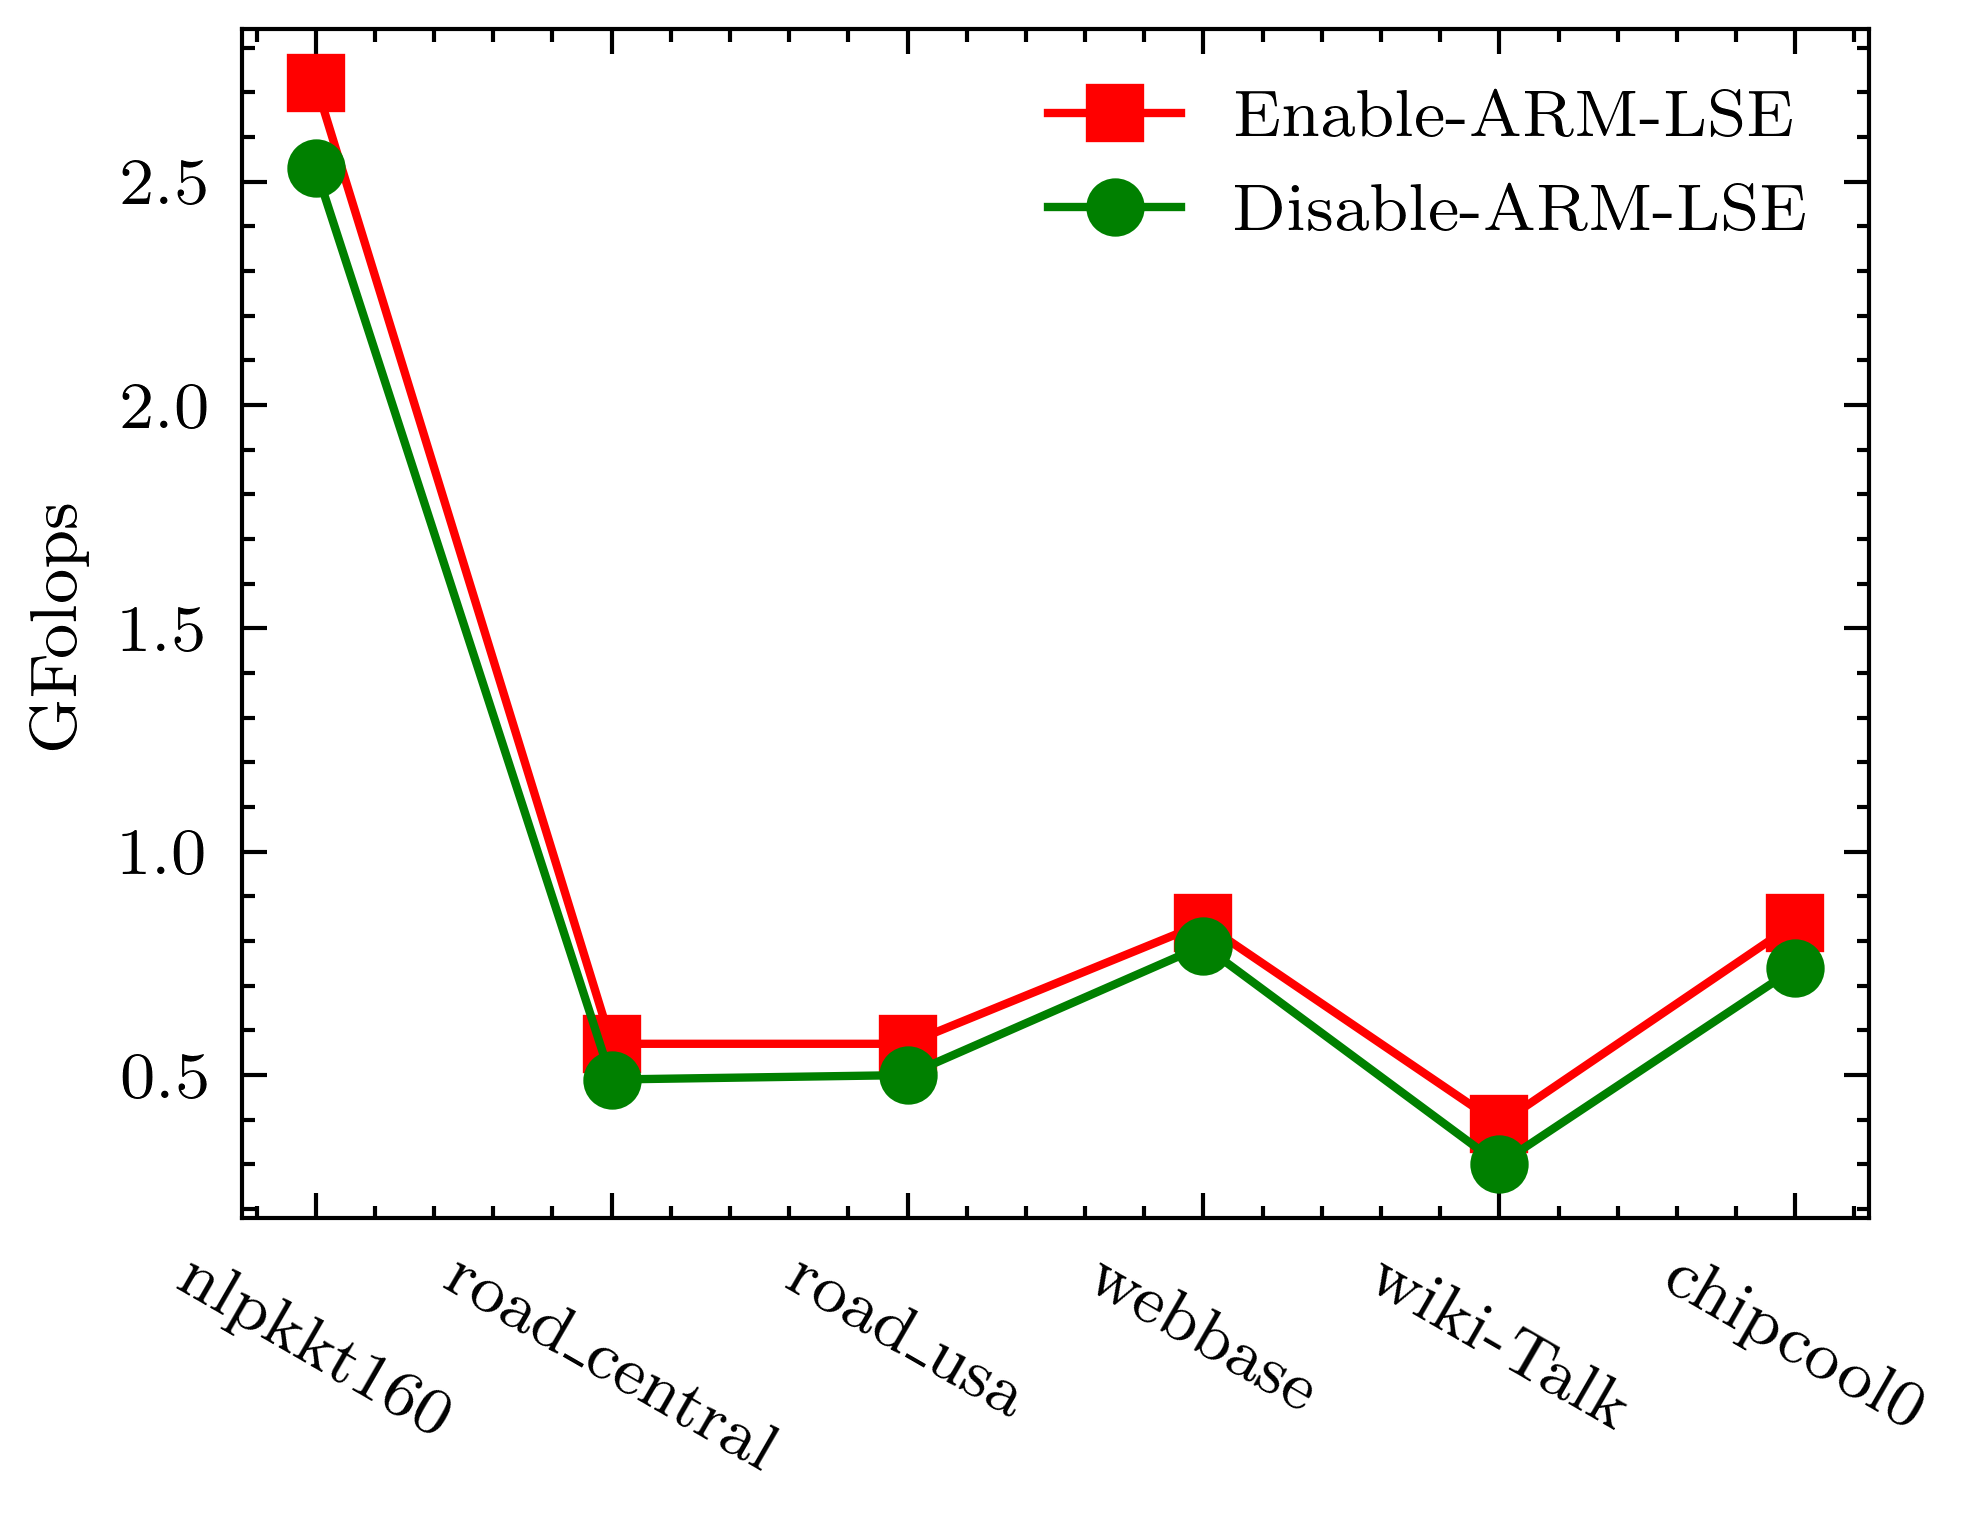
\includegraphics[width=0.7\textwidth]{ARMLSETEST.png}
    \caption{测试ARMv8原子指令对性能的影响}
    \label{测试ARMv8原子指令对性能的影响}
\end{figure}

图\ref{测试ARMv8原子指令对性能的影响}展示了ARMv8原子指令对算法性能的影响。在使用了ARMv8原子指令之后,性能相比于ARM传统的原子指令,性能有所提升。

\section{NUMA架构对性能的影响}\label{NUMA架构对性能的影响}

对于绝大多数的矩阵使用numctl命令将计算放到结点的内部,计算效率是最高的。但是对于规模较大,并行性较好的矩阵,将任务分配到两个NUMA结点上相比于单节点能够获得约10\%的性能提升。

\begin{figure}[htbp]
    \centering
    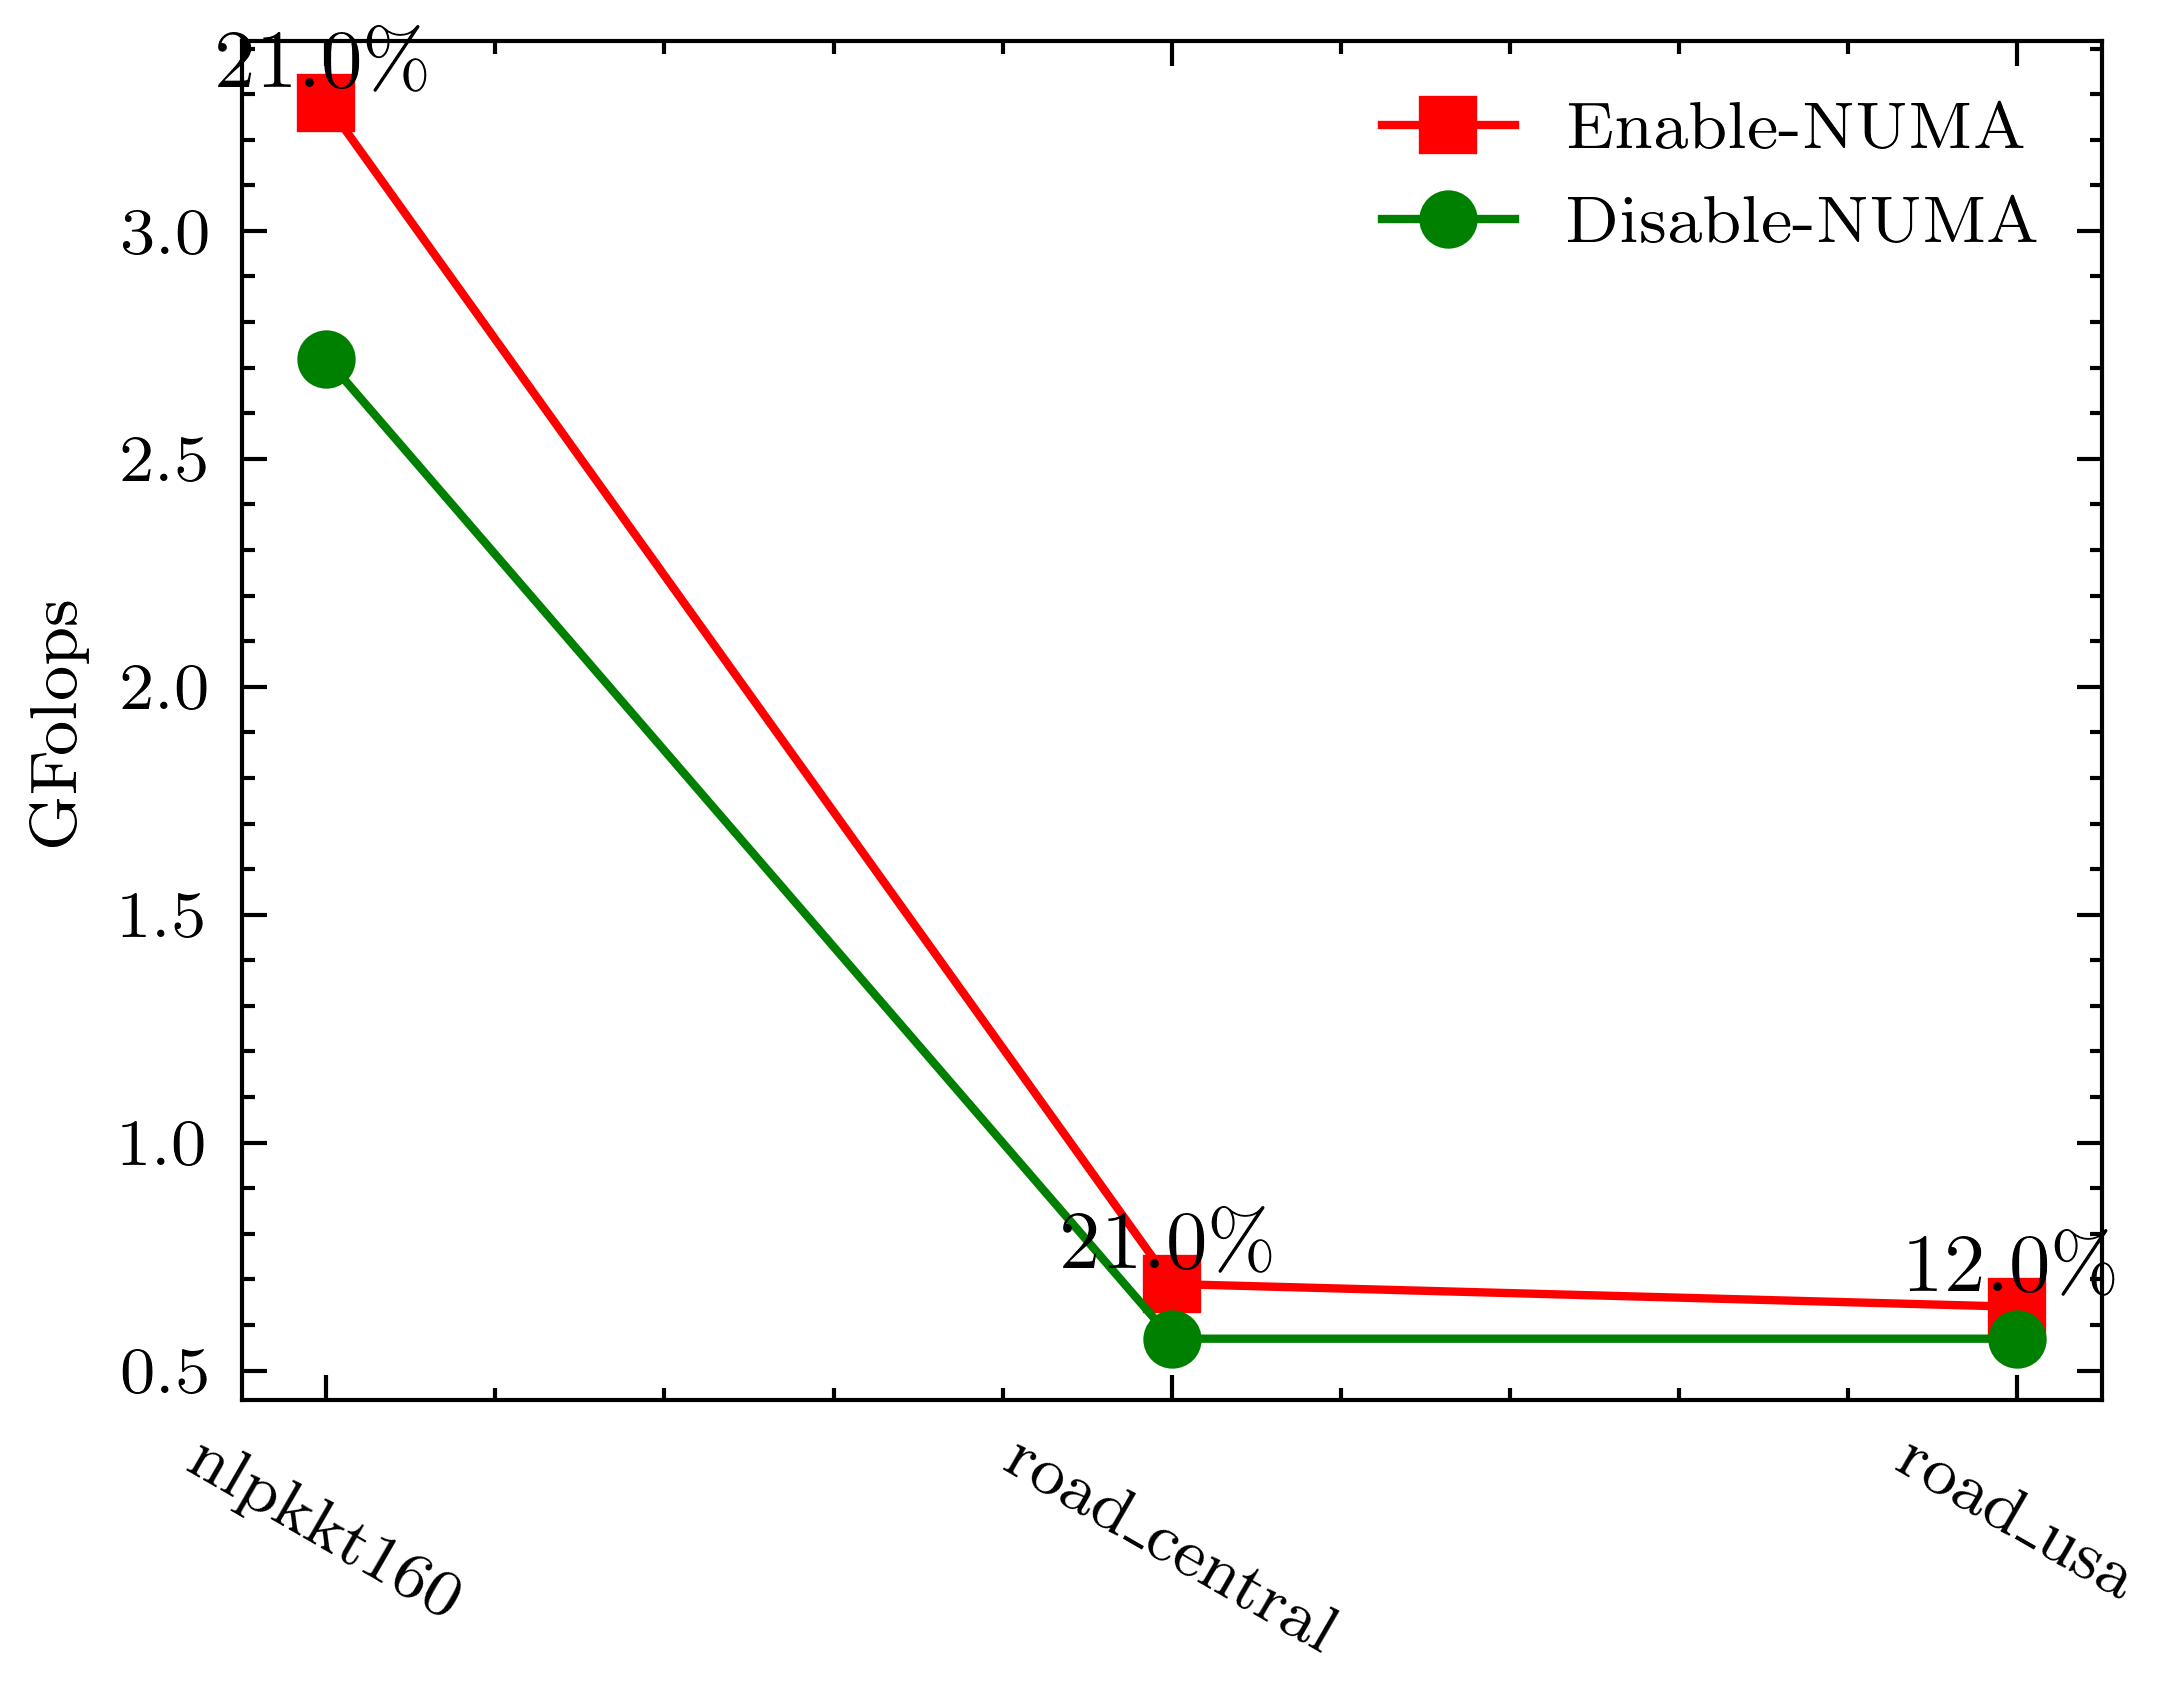
\includegraphics[width=0.7\textwidth]{NUMATEST.png}
    \caption{测试NUMA架构对性能的影响}
    \label{测试NUMA架构对性能的影响}
\end{figure}

如图\ref{测试NUMA架构对性能的影响},将cscRowPtr[]、cscColIdx[]、cscVal[]、b[],以只读数据副本的形式分配到两个NUMA结点并启用两个NUMA结点的核心之后,nlpkkt160、road\_central、road\_usa这三个规模较大的稀疏矩阵能够分别获得约21\%、21\%以及12\%的加速比。

对于规模较小或者并行性较低的矩阵,仅仅只用一个结点运行,性能更好,对于规模较大的矩阵使用多个NUMA节点进行运算能够获得更好的性能。

\section{本章总结}

本章测试分析了本文提出的SpTRSV算法的性能,并与其他平台现有的SpTRSV算法性能进行了对比,见图\ref{MatrixSuite}。同时也测试分析了算法在预处理阶段和计算阶段分别占用的时间,见表\ref{算法耗时分解表},相比于基于level-sets的算法,本文提出的SpTRSV算法的预处理时间大大减少。最后说明了本文所使用的几个优化技巧对性能的提升效果,例如使用负载均衡优化能够获得约平均23\%的性能提升、使用ARM原子指令和CPU松弛优化后一共能够获得平均10.5\%左右的性能提升、对于大规模稀疏矩阵使用NUMA架构的优化,能够获得平均约18\%的性能提升。


\endinput